% Generated by build_manuscript.py from 03_framework.md
\section{3 Task-driven multimodal inspection framework}\label{task-driven-multimodal-inspection-framework}

\subsection{3.1 Problem formulation}\label{problem-formulation}

The inspection task is to acquire a limited subset of an internal C-scan image while maintaining an estimate of compression-after-impact (CAI) strength. For each specimen, let S denote the available surface image, X the internal image, and y the measured CAI strength in MPa. We partition each image into an 8×8 grid with index set I=\{1,\ldots,64\}. An action acquires one previously unobserved internal cell. Thus, the decision concerns a region of an existing image in offline replay; it does not specify an individual acoustic waveform, probe displacement or physical scan command. The surface image is available before internal acquisition begins.

After t actions, the observed set is \(\Omega_t\) and its binary indicator is \(M_t\). The cumulative acquisition fraction \(c_t\) is the number of unique acquired native image pixels divided by the number of pixels in the complete internal image. Grid boundaries are rounded on the native image, so cell costs need not be identical. We retain these actual pixel counts when checking affordability and evaluating a trajectory. With B=0.25, the legal action set contains only unobserved cells whose complete acquisition keeps \(c_t\) within B. Acquisition ends when this set is empty. This rule defines a budget-limited experiment without a learned stopping decision.

A frozen predictor produces \(\hat{y}_t=P_{\mathrm{all}}(S,M_t\odot X,M_t,c_t)\). The policy selects the next cell from the currently legal set using surface information and, for feedback policies, the acquired internal evidence and current prediction. The true strength y is available to training and retrospective scoring, but is excluded from the decision state. This separation allows the acquisition policy to be trained for a downstream assessment objective without supplying the answer when selecting an observation. The comparison then asks which policy supplies a useful sequence of observations to the same predictor.

We evaluate both the trajectory and its final estimate. Let \(e_t=|\hat{y}_t-y|\) and let e(c) hold the most recently available error constant until the next acquisition completes. The normalized trajectory error and objective are

\[A(B)=\frac{1}{B}\int_0^B e(c)\,dc,\qquad J=A(B)+0.25e_T.\]

Both terms are measured in MPa and lower values are preferable. A(B) measures prediction quality over the available acquisition range, whereas the terminal term retains an explicit incentive for final quality. The last prediction is held from \(c_T\) to B if no remaining whole cell is affordable. Consequently, a trajectory cannot avoid its final holding cost by ending below the cap. This formulation couples what is acquired with when its effect becomes available.

\begin{figure}
\centering
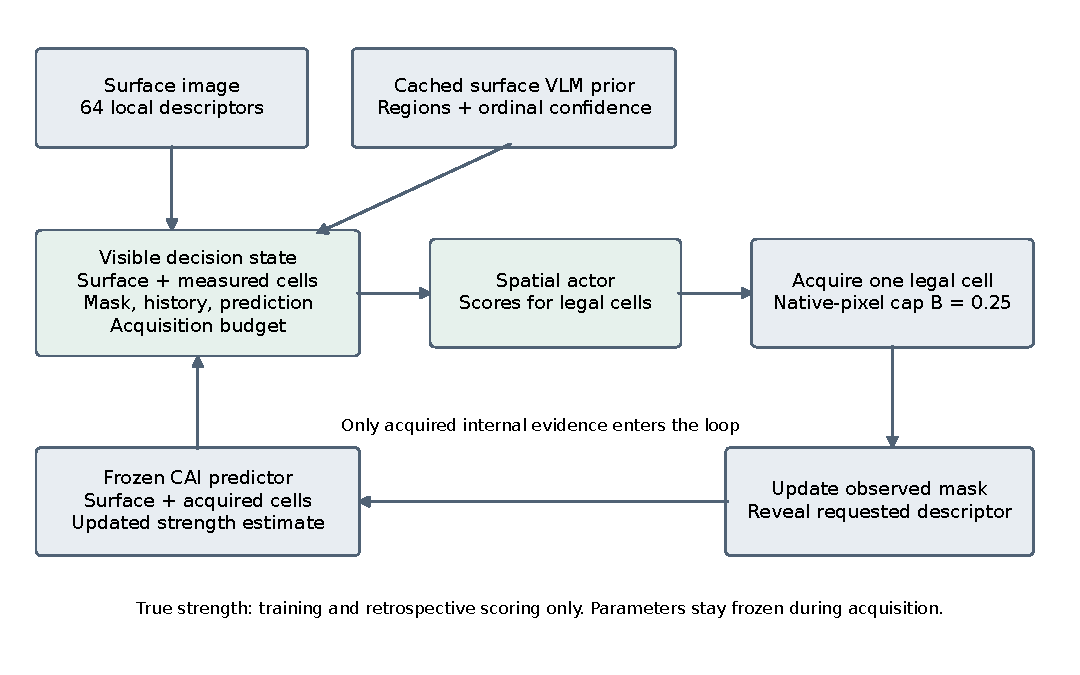
\includegraphics[width=1\linewidth,height=\textheight,keepaspectratio,alt={Multimodal acquisition workflow. Only requested internal descriptors enter the visible state. The frozen VLM supplies a cached surface prior; the actor makes each acquisition decision. Codex (GPT-6, OpenAI) assisted in writing the deterministic plotting code; author scientific review is pending.}]{figures/Fig1_framework.pdf}
\caption{Multimodal acquisition workflow. Only requested internal descriptors enter the visible state. The frozen VLM supplies a cached surface prior; the actor makes each acquisition decision. Codex (GPT-6, OpenAI) assisted in writing the deterministic plotting code; author scientific review is pending.}\label{fig:framework}
\end{figure}

\subsection{3.2 Multimodal inspection-state representation}\label{multimodal-inspection-state-representation}

A consistent spatial representation connects surface cues to candidate internal observations. Frozen ResNet18 encoders \citep{he2015} produce a 512-dimensional descriptor for each of the 64 cells in each modality. Each cell is cropped before encoding, rather than extracted from a whole-image feature map that may already mix information across internal regions. The resulting surface and internal feature arrays each have shape 64×512. Corresponding grid coordinates are normalized to {[}0,1{]} in the row and column directions. These coordinates provide an explicit location reference for the predictor and acquisition policy; they do not establish a mechanically calibrated three-dimensional damage map.

Offline replay stores the complete internal feature array on the environment side so that any legal requested cell can be revealed. Model visibility is narrower than storage availability. Before cell mixing or spatial interaction, the predictor replaces unknown internal content with zero, and the spatial feedback actor replaces it with a learned mask vector. The binary observed flag distinguishes unknown cells from measured cells. Surface descriptors remain available everywhere. The actor also receives acquisition history and remaining budget, enabling it to distinguish a region that has not been visited from one that has already contributed to the current estimate.

A frozen Qwen2.5-VL-7B-Instruct model \citep{bai2025} supplies an additional surface prior. It examines clean and gridded surface views and returns candidate regions, ordinal confidence and cue-availability information. The acquisition actor receives numerical region indicators and confidence features, not the full generated explanation. Confidence is mapped from unknown, low, medium and high to 0, 1/3, 2/3 and 1, respectively; overlapping regions retain the highest confidence for a cell. These values encode an ordering of reported confidence rather than calibrated probabilities of internal damage. The VLM does not observe the hidden internal image, estimate CAI strength or produce a fresh language plan at every acquisition step.

The prior has a specific initialization role. At the first action, cells in the highest available reliable confidence level, restricted to medium or high, form a candidate set C0. The policy scores the affordable legal cells within that set. If the VLM is unavailable, reports no reliable cue, supplies no reliable region or leaves no affordable candidate, the ordinary legal set is retained. After the first acquisition, this hard restriction is removed while the numerical VLM features remain in the actor state. This design makes the initial prior explicit without constraining the entire sequence to a surface-selected region. Unavailability and an available response reporting no reliable cue are represented separately.

The information boundary can be summarized as follows.

{ % do not increment counter
\begin{center}\begin{minipage}{\linewidth}\small
\begin{tabular}{@{}
  >{\raggedright\arraybackslash}p{(\linewidth - 6\tabcolsep) * \real{0.2500}}
  >{\raggedright\arraybackslash}p{(\linewidth - 6\tabcolsep) * \real{0.2500}}
  >{\raggedright\arraybackslash}p{(\linewidth - 6\tabcolsep) * \real{0.2500}}
  >{\raggedright\arraybackslash}p{(\linewidth - 6\tabcolsep) * \real{0.2500}}@{}}
\toprule\noalign{}
\begin{minipage}[b]{\linewidth}\raggedright
Information
\end{minipage} & \begin{minipage}[b]{\linewidth}\raggedright
Acquisition actor during evaluation
\end{minipage} & \begin{minipage}[b]{\linewidth}\raggedright
Frozen CAI predictor
\end{minipage} & \begin{minipage}[b]{\linewidth}\raggedright
Training/scoring side
\end{minipage} \\
\midrule\noalign{}



Complete surface descriptors & Available & Available & Available \\
Surface VLM region features & Available in VLM variants & Not an input & Available \\
Acquired internal descriptors & Available in feedback variants & Available & Available \\
Unacquired internal descriptors & Hidden & Hidden & Stored only by replay environment \\
Observed mask and acquisition fraction & Available & Available & Available \\
Action history and remaining budget & Available to state-dependent policies & Not an input & Available \\
Current predicted CAI strength & Available in feedback variants & Output & Available \\
True CAI strength & Excluded & Excluded from input & Supervision and scoring only \\
\bottomrule\end{tabular}
\end{minipage}\end{center}
}

\subsection{3.3 Partial-observation CAI assessment}\label{partial-observation-cai-assessment}

A common assessment model is necessary to distinguish acquisition choices from changes in the downstream regressor. All nine strategies are evaluated with the same selected MEAN\_SC predictor. Surface and masked internal descriptors are separately projected to 64 dimensions. For each cell, their concatenation with its observed indicator and two coordinates passes through a two-layer cell multilayer perceptron with GELU activations. This yields a 64-dimensional cell representation that contains local surface information and, where measured, internal information.

The predictor forms two summaries: the mean over all 64 fused cell representations and the mean over measured cells. The measured mean uses a denominator bounded below by one, which makes the initial empty state well defined. The all-cell mean is not a surface-only branch: measured internal content is already present in its constituent cell representations. Concatenating both summaries with the actual acquisition fraction gives the regression-head input. The normalized output is transformed to MPa using the training-derived target mean and scale. The same computation accepts an empty internal set, a partially observed set or all 64 cells.

Neither the policy identifier nor the acquisition order enters this predictor. Therefore, for the same surface, observed cells and cost, its output is identical regardless of the policy that produced the state. Different acquisition sequences can still have different A(B), even when they eventually reveal the same subset, because intermediate predictions are available at different costs. This property gives the trajectory comparison its interpretation: changes in prediction quality arise through supplied observations and their timing, under a fixed assessment mapping.

The predictor used for reported validation results was selected at update 1750 and then frozen. During policy learning, rewards instead use three frozen cross-fitted predictors. Each training specimen is evaluated by the model assigned to its fold, trained with its capture group excluded. These models provide out-of-fold training feedback; they are not averaged into a three-model ensemble for the reported validation predictions. The complete-input reference also uses the common selected predictor, with all internal cells and the same surface information.

\subsection{3.4 State-dependent acquisition policy}\label{state-dependent-acquisition-policy}

The spatial actor represents each candidate location jointly with the current assessment state. Surface and visible internal descriptors are each projected to 48 dimensions. Their concatenation with row and column coordinates, the observed flag, normalized action history, VLM region indicator and confidence is mapped to a 128-dimensional cell token. A separate query token represents cumulative cost, remaining budget, normalized current CAI prediction, VLM availability, the no-reliable-cue indicator and the fraction of observed cells. These 65 tokens pass through two Transformer encoder layers \citep{vaswani2017} with four attention heads and a feed-forward width of 256.

The resulting query representation supplies global context to every cell. An action head scores each concatenated contextual cell and query pair; illegal cells are excluded before selection. A separate value head estimates the remaining training cost from the query representation. The value head is a critic used to reduce policy-gradient variation, not the predictor of reported CAI strength. The architecture thus connects a local choice to the current observation set while retaining a distinct assessment model. Its spatial interactions operate on already masked features, so the global context cannot retrieve hidden internal content through attention.

Policy-gradient learning \citep{williams1992} minimizes the expected trajectory objective over training specimens and sampled actions. Specimens are sampled by first choosing a domain uniformly and then a physical specimen within that domain. For each trajectory, the frozen cross-fitted predictor supplies absolute errors used to construct cost-to-go targets. The actor loss sums log action probabilities weighted by detached cost-to-go minus the critic estimate; a squared-error critic loss with weight 0.5 and an entropy term complete the optimization objective. Costs are normalized by the existing training target scale, and the discount factor is one. The shared static policy uses a zero baseline. This is task-loss-based policy learning, without an action-demonstration target.

During training, actions are sampled from the legal categorical distribution. During evaluation, the highest-scoring legal action is selected and the actor is evaluated again after the observation update. Parameters remain frozen during this sequence. The open-loop diagnostic removes internal descriptors and the current prediction from the decision computation but retains surface features, location, prior, acquisition history and budget. Its downstream predictor still incorporates the acquired internal information. The no-VLM diagnostic retains surface and internal feedback while removing the VLM features and initial restriction. These distinctions separate the information used to choose a cell from that used to assess the specimen afterwards.

\textbf{Algorithm 1. Budget-limited task-driven acquisition}

\begin{verbatim}
Input: surface features S, cached surface prior V, frozen actor pi and predictor P
Set observed mask M=0, history H=0 and native-pixel cost c=0
Compute the initial CAI prediction p=P(S, masked_X, M, c)
Repeat:
    Construct L from unobserved cells affordable under B=0.25
    If L is empty, terminate
    On the first step, restrict L to the highest reliable C0 if feasible
    Build the permitted actor state from S, V, M, H, p and budget
    Score legal cells and choose a=argmax pi(state) over L
    Reveal internal descriptor X[a] from the replay environment
    Update M, H and c using the newly acquired native pixels
    Update p=P(S, masked_X, M, c)
    Record the state and proceed with unchanged model parameters
Return the acquisition sequence and partial-observation predictions
Use y only outside this loop to calculate evaluation errors
\end{verbatim}

\subsection{3.5 Acquisition timing and task cost}\label{acquisition-timing-and-task-cost}

The trajectory objective admits a direct decomposition using saved prediction changes. For an acquisition completed at \(c_t\), define \(\delta_t=e_{t-1}-e_t\) and

\[g_t=(1-c_t/B)\,\delta_t,\qquad A(B)=e_0-\sum_{t=1}^{T}g_t.\]

An error reduction contributes in proportion to the budget interval over which its updated prediction can influence the trajectory area. An error increase produces a negative contribution and is retained. An observation completed exactly at B has zero contribution to A(B), although its prediction change can affect the terminal term in J. The identity also includes the holding interval after a trajectory ends below B; no additional extrapolated observations are required. Supplementary material gives the telescoping derivation.

For descriptive analysis, we group these signed contributions by acquisition completion stage: (0,0.0625{]}, (0.0625,0.125{]}, (0.125,0.1875{]} and (0.1875,0.25{]}. A contribution assigned to a stage measures its weighted effect over the remaining budget, rather than an improvement confined to that stage's integration interval. Aggregating first within an episode, then across repeated runs of each specimen, within domains and equally across domains preserves the estimand used for A. This is an accounting identity for the observed loss, not a causal allocation of gains to components or a new intervention on the acquisition policy.
